\section{Regulador experto}
\label{sec:reg_expt}

Durante las producciones realizadas anteriormente, se ha notado que existe una relación entre la velocidad de tracción y el diámetro final del filamento, sin embargo, el sistema que se dispone carece de la robustez necesaria para poder trabajar con un regulador del tipo PID, en el que es necesario conocer de manera lo más exacta posible, la distribución de la planta con la que se trabaja.\\

Como se ha visto en los ensayos anteriores, la salida de filamento que proporciona el filastruder no es constante y en ocasiones, no está bien mezclada.

\begin{figure}[H]
    \centering
    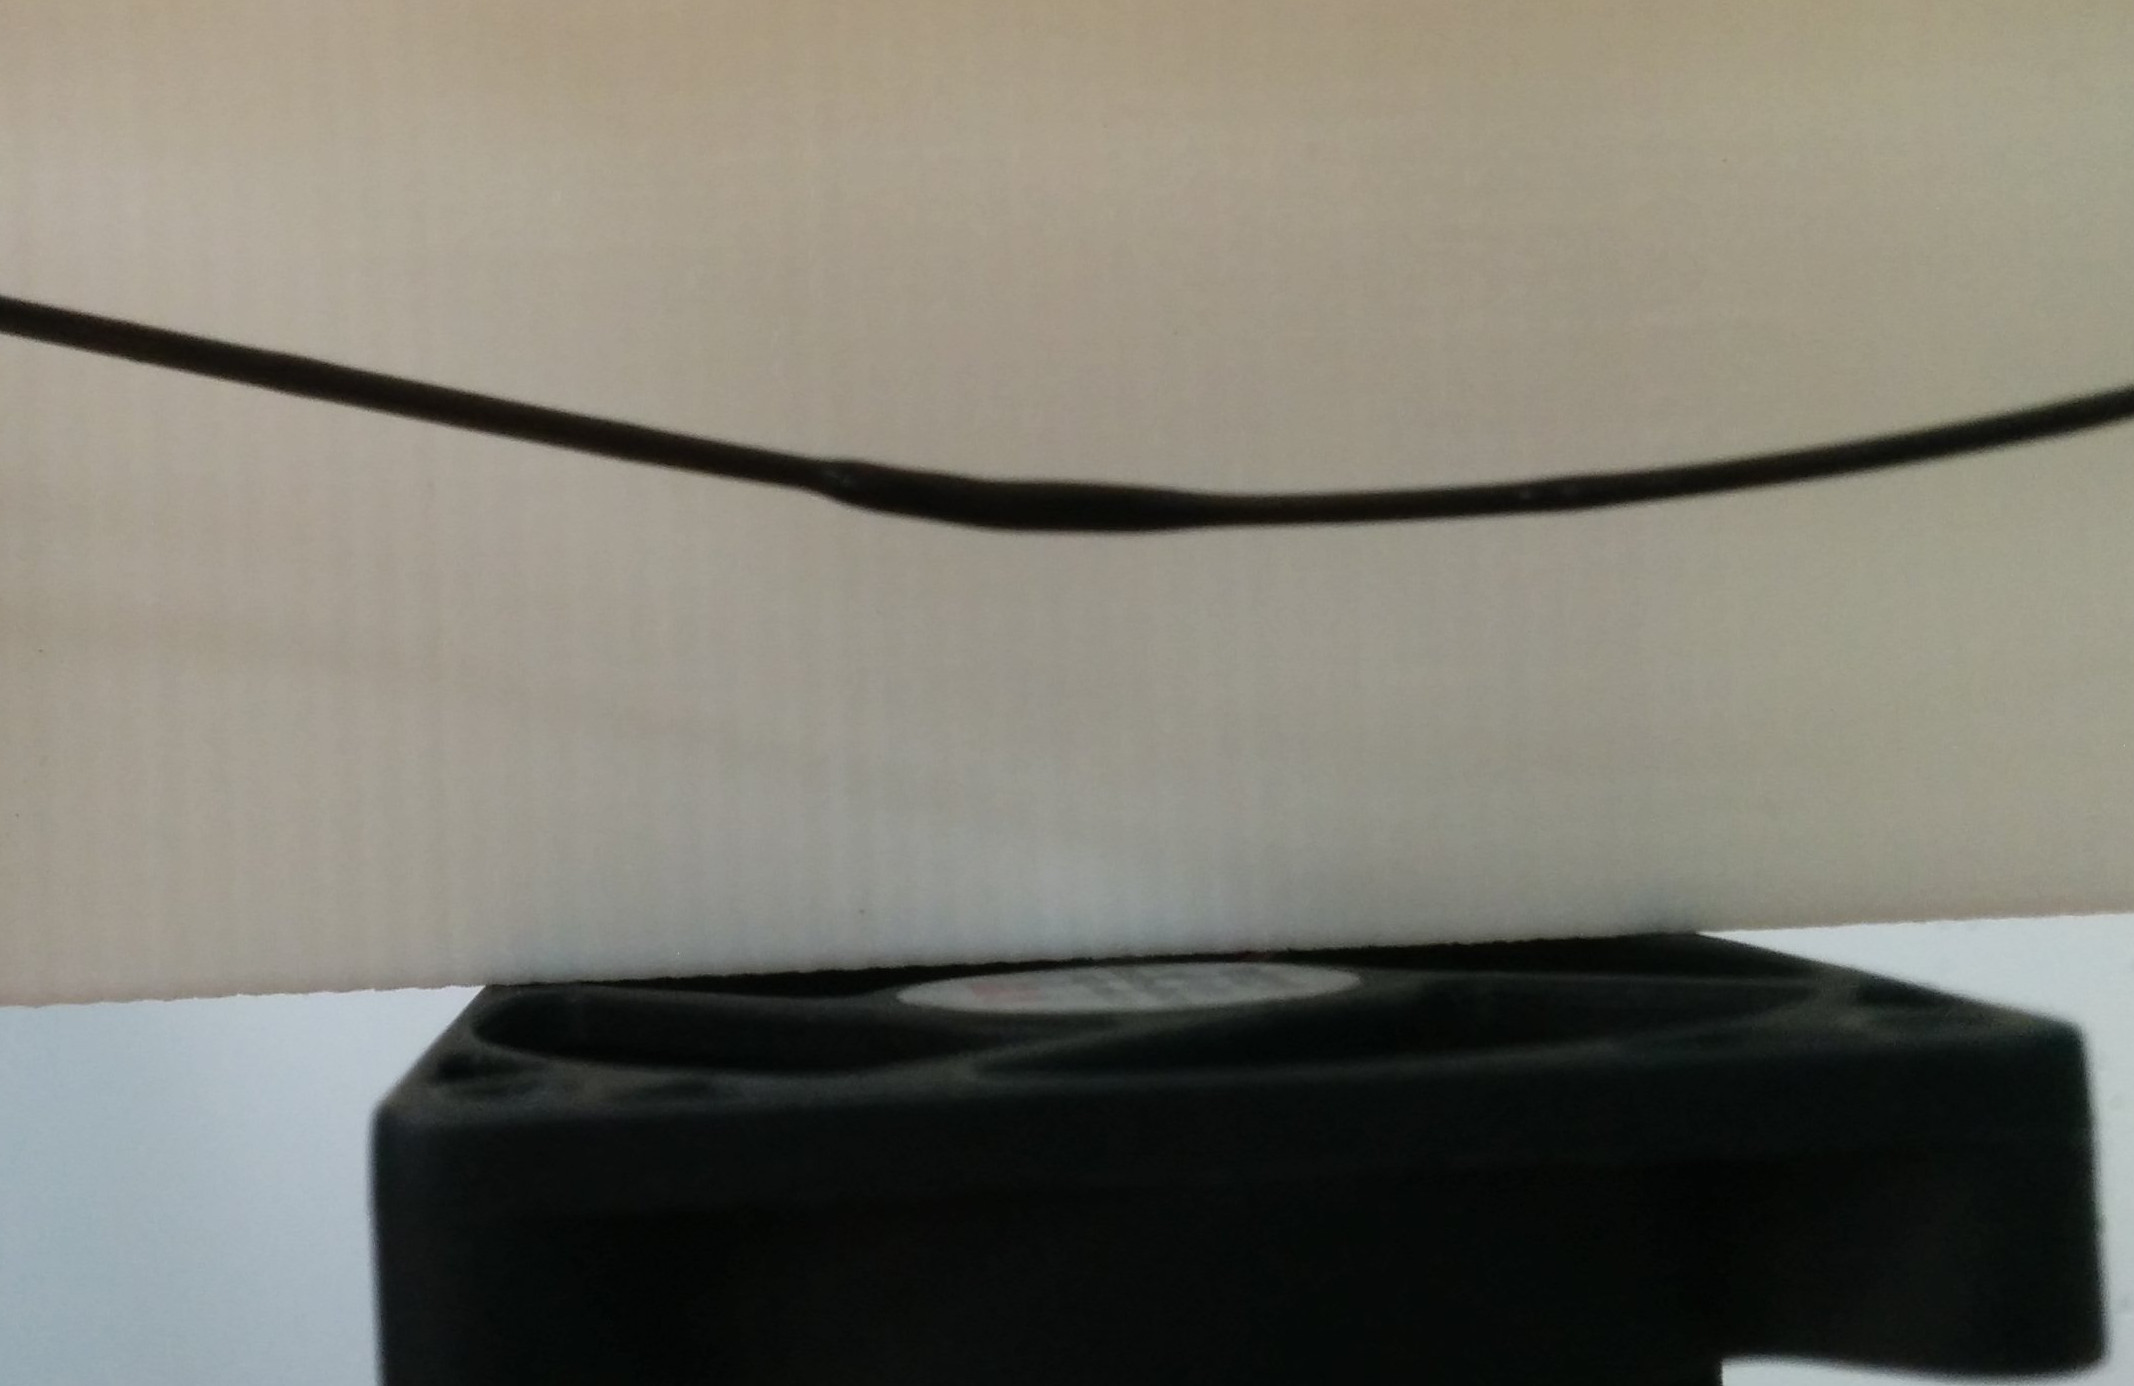
\includegraphics[width=0.6\textwidth]{images/producciones/22072015/IMG_20150722_120959.jpg}
    \caption{Mezcla incorrecta de la filastruder}
    \label{fig:reg_mezcla}
\end{figure}

Por ello, se decide no usar un regulador PID e intentar implementar un regulador experto, el cual, imitará las acciones que un humano tomaría para resolver el problema. Este tipo de reguladores se basan en un conocimiento previamente adquirido por una persona, que ha trabajado con el sistema.\\

Para implementear este sistema, se definen una serie de reglas, en las que acotaremos los diámetros del filamento en regiones, y dependiendo, de si el diámetro crece o decerece, se actuará sobre la velocidad de tracción